\documentclass{article}
\usepackage{microtype,graphicx,booktabs,amsmath,amssymb,hyperref}
\newcommand{\theHalgorithm}{\arabic{algorithm}}
\usepackage{icml2021}
\icmltitlerunning{Beyond Polynomial Expansion: Revisiting Kryptonite-3.0}
\begin{document}
\setcounter{dbltopnumber}{1}
\raggedbottom
\twocolumn[
\icmltitle{Beyond Polynomial Expansion: Revisiting Kryptonite-3.0 Through Representation, Data Scaling, and Low-Rank Adaptation}
\begin{icmlauthorlist}
\icmlauthor{Charlie Wang, Zihao Zhao, Jerry Li, William Chia}{imp}
\end{icmlauthorlist}
\icmlaffiliation{imp}{Imperial College London, London, United Kingdom}
\icmlcorrespondingauthor{Coursework team}{No email given}
\vskip 0.3in
]
\printAffiliationsAndNotice{}
\footnotetext{Development repository: \url{https://github.com/jerryliruijie/Kryptonite_v3.0}. Submission GitLab URL and final reproducible commit remain to be supplied.}

\begin{abstract}
Kryptonite-3.0 uses the failure of selected classifiers and frozen pretrained representations to argue that its tasks resist modern machine learning. We revisit this conclusion with sign-transformed CatBoost, scratch MLPs, matched learning curves, and low-rank adaptation (LoRA) of KryptoNet-40. After local validation-based selection and refitting on 90\% of the labelled data, sign-CatBoost achieves 93.44--96.28\% mean local-test accuracy on Kryptonite-20, -30 and -40, compared with 53.41--54.50\% for quadratic logistic regression. Increasing the matched training subsets fourfold improves CatBoost validation accuracy by 5.89--13.32 percentage points, whereas quadratic logistic regression gains at most 2.46 points. On Kryptonite-40-Adapt, validation-selected rank-1 LoRA reaches 95.75\% mean local-test accuracy while training 0.51\% of the network's parameters. These results challenge the mock paper's general inference for the evaluated methods; they do not establish performance on the hidden sets.
\end{abstract}

\section{Introduction}
Challenge datasets evaluate the capabilities of machine learning models. A model's performance depends on its expressive capacity, the effectiveness of optimization, and its ability to generalize to unseen data. Universal approximation theorems establish that certain neural networks can approximate a broad class of functions \cite{leshno1993}.

Kryptonite-3.0 \cite{quinn2026} challenges the effectiveness of machine learning through three main findings. First, polynomial logistic regression achieves less than 59\% accuracy even with polynomial features of degree 10, which the authors interpret as evidence against universal approximation. Second, quadrupling the training data produces only marginal improvements in quadratic logistic regression, leading the authors to question whether additional data can solve these tasks. Third, despite achieving 95\% accuracy on its pretraining task, KryptoNet-40 performs poorly under zero-shot evaluation and frozen-representation probing. These experiments motivate the study of additional models and adaptation strategies.

We investigate alternative classification methods, the effects of training-set size, and parameter-efficient adaptation. We compare logistic regression baselines with gradient-boosted decision trees and multilayer perceptrons (MLPs) trained from scratch. We combine a sign-based input representation with CatBoost to classify the three main Kryptonite datasets. We examine the relationship between training-set size and generalization by comparing learning curves on identical training subsets. We also apply low-rank adaptation (LoRA) to KryptoNet-40, allowing its internal representations to be updated while keeping the pretrained hidden weights frozen.

Our main contributions are threefold:

\begin{enumerate}
\item \textbf{Representation-aware classification.} Sign-based CatBoost exceeds 90\% local-test accuracy on each of the three main Kryptonite datasets.
\item \textbf{Model-dependent data scaling.} Matched learning curves show larger gains from increasing the training data for sign-transformed CatBoost than for quadratic logistic regression.
\item \textbf{Parameter-efficient adaptation.} We demonstrate effective LoRA adaptation of KryptoNet-40 under the evaluated setting and analyze its trainable parameter count and computational complexity relative to full fine-tuning.
\end{enumerate}

\section{Methodology}
\subsection{Classification objective and polynomial controls}
For labelled observations $\mathcal D=\{(x_j,y_j)\}_{j=1}^m$, with $x_j\in\mathbb R^d$ and $y_j\in\{0,1\}$, a model produces a logit $z_\theta(x)$ and probability $p_\theta(x)=\sigma(z_\theta(x))$, where $\sigma(z)=(1+e^{-z})^{-1}$. We minimize binary cross-entropy,
\begin{equation}
\mathcal L=-\frac1m\sum_{j=1}^m\left[y_j\log p_j+(1-y_j)\log(1-p_j)\right].
\label{eq:bce}
\end{equation}
Logistic regression uses $z_\theta(x)=w^\top\phi(x)+b$. The linear control sets $\phi(x)=x$; the quadratic control includes the original coordinates and all products $x_i x_k$ for $i\leq k$. Its feature dimension is $d+d(d+1)/2$, excluding the intercept. Both use L2-regularized log loss, inverse regularization strength $C=0.85$, and L-BFGS with at most 1,000 iterations and tolerance $10^{-6}$. A training-majority classifier checks the approximately balanced task. The controls use the shared split; Kryptonite-3.0 evaluates a normalized degree-1--10 kernel.

\subsection{Sign-based CatBoost}
We use a binary representation of each input feature based on its sign. Sign-based binary representations have been studied for classification \cite{needell2018}. The starter implementation accompanying Kryptonite-3.0 also applies a sign transformation before its polynomial kernel \cite{quinn2026}. We combine sign-transformed inputs with CatBoost to learn interactions between feature signs. For an input $x\in\mathbb R^d$, we set
\begin{equation}
s_i(x)=\begin{cases}+1,&x_i\geq0,\\-1,&x_i<0.\end{cases}
\label{eq:sign}
\end{equation}
CatBoost \cite{prokhorenkova2018} combines decision trees in an additive model. Given the sign-transformed input, the logit and predicted probability are
\begin{align}
F_t(s)&=F_{t-1}(s)+\eta T_t(s),\nonumber\\
p(x)&=\sigma(F_T(s(x))).
\end{align}
Here $T_t$ is the tree added at iteration $t$ and $\eta$ controls its contribution. Let $\ell_j$ be the per-example binary cross-entropy in Equation~\ref{eq:bce} and $p_{j,t-1}=\sigma(F_{t-1}(s(x_j)))$. Its negative gradient with respect to the current logit is
\begin{equation}
-\frac{\partial\ell_j}{\partial F_{t-1}(s(x_j))}=y_j-p_{j,t-1}.
\end{equation}
CatBoost uses gradient information to construct each tree and estimate its leaf values. Each symmetric tree applies the same split at a given depth. A path through the tree combines conditions on the signs of features, and its leaf value contributes to the logit. We use 600 symmetric trees of depth 10, a learning rate $\eta=0.05$, and leaf L2 regularization 10. A depth-10 tree has at most $2^{10}=1024$ leaves. The final prediction is class 1 when $p(x)>0.5$ and class 0 otherwise.

\subsection{MLPs and optimization}
The scratch MLP uses two ReLU hidden layers of equal width $h\in\{128,256\}$:
\begin{align}
h_1&=\operatorname{ReLU}(W_1\tilde x+b_1),\nonumber\\
h_2&=\operatorname{ReLU}(W_2h_1+b_2),\qquad z=w^\top h_2+b.
\end{align}
Here $\tilde x_i=(x_i-\mu_i)/\sigma_i$, with statistics fitted only on training rows. The model retains continuous magnitudes and learns a nonlinear representation, providing a complementary test to sign-based trees.

Adam \cite{kingma2015} uses gradient $g_t$, moment estimates $u_t=\beta_1u_{t-1}+(1-\beta_1)g_t$ and $v_t=\beta_2v_{t-1}+(1-\beta_2)g_t^2$, and the elementwise update
\begin{align}
\hat u_t&=\frac{u_t}{1-\beta_1^t},\qquad \hat v_t=\frac{v_t}{1-\beta_2^t},\nonumber\\
\theta_{t+1}&=\theta_t-\eta\frac{\hat u_t}{\sqrt{\hat v_t}+\epsilon}.
\end{align}
We use $(\beta_1,\beta_2)=(0.9,0.999)$, $\epsilon=10^{-8}$, $\eta=10^{-3}$ and batch size 256. Coupled weight decay adds $10^{-4}\theta_t$ to the loss gradient. During initial development, training ran for at most 150 epochs, with a minimum of 30 and patience 20 for validation-accuracy improvement. The checkpoint maximized validation accuracy, with lower validation loss breaking ties.

\subsection{Low-rank adaptation of KryptoNet-40}
KryptoNet-40 has four width-512 ReLU hidden layers and a scalar output head, totalling 809,473 parameters. For a pretrained layer $W\in\mathbb R^{o\times i}$, LoRA \cite{hu2022} computes
\begin{equation}
Y=WX+b\mathbf1^\top+sBAX,\qquad s=\alpha/r,
\label{eq:lora}
\end{equation}
where $X\in\mathbb R^{i\times N}$, $A\in\mathbb R^{r\times i}$ and $B\in\mathbb R^{o\times r}$. We freeze $W,b$, initialize $A$ with Kaiming-uniform values and $B$ to zero, and train $A,B$. Thus the initial layer equals its pretrained counterpart, while $\operatorname{rank}(BA)\leq r$ constrains the update. The rank sets the width of the bottleneck through which the update acts: $AX$ projects each input onto $r$ directions, and $B$ maps them back to the output space. Thus $r$ controls both the update's capacity and its $r(i+o)$ trainable parameters, and a small $r$ acts as a regularizer. We fix $\alpha=8$ for every rank, so $s=8/r$. We adapt all four hidden layers and train the existing output head, using raw inputs.

LoRA and the linear probe use Adam with the default $\beta$ and $\epsilon$ of Section~2.3, no weight decay and batch size 128. The learning rate is $10^{-3}$ for LoRA and $10^{-2}$ for the probe, whose head is reinitialized. During initial development, training used at most 300 epochs and patience 40. The checkpoint maximized validation accuracy, with lower validation loss breaking ties; an improvement of either kind reset the patience counter.

Writing $Z=AX$ and $G=\partial\mathcal L/\partial Y$, backpropagation gives
\begin{align}
\nabla_B\mathcal L&=sGZ^\top,& G_Z&=sB^\top G,\nonumber\\
\nabla_A\mathcal L&=G_ZX^\top,&\nabla_X\mathcal L&=W^\top G+A^\top G_Z.
\label{eq:gradients}
\end{align}
Initially $\nabla_A\mathcal L=0$, but $B$ can receive a nonzero gradient. Freezing $W$ removes its parameter gradient, while $W^\top G$ propagates gradients to earlier trainable layers.

\subsection{Training-step operation counts}
We count an $n\times m$ by $m\times k$ product as $nmk$ operations. One step means a forward and backward pass over $N$ inputs; bias additions, nonlinearities, scalar operations and optimizer updates are excluded. Full fine-tuning trains $oi+o$ parameters, including bias, and costs $3oiN$ if an input gradient is needed: $WX$, $GX^\top$ and $W^\top G$.

Evaluating $B(AX)$ and caching $Z$ costs $oiN+rN(i+o)$ forward operations. The parameter and intermediate gradients in Equation~\ref{eq:gradients} cost $rN(i+2o)$, and the input gradient costs $oiN+irN$. Consequently,
\begin{equation}
C_{\mathrm{LoRA}}=2oiN+3rN(i+o),\qquad
P_{\mathrm{LoRA}}=r(i+o).
\label{eq:cost}
\end{equation}
If the input gradient is unnecessary, the full and LoRA costs become $2oiN$ and $oiN+rN(2i+3o)$, respectively. The latter applies to the first hidden layer when the input data require no gradient.

Product order matters in both passes. Forming $(BA)X$ costs $oir+oiN$ for the update alone, instead of $rN(i+o)$ for $B(AX)$. Similarly, computing $\nabla_A\mathcal L$ as $s(B^\top G)X^\top$ costs $rN(o+i)$, whereas $sB^\top(GX^\top)$ costs $oiN+roi$. Reusing $Z$ in $GZ^\top$ also avoids a dense intermediate. Efficient order depends on the dimensions and cached products; the factored order is appropriate for our small ranks.

Including the trainable 513-parameter head, the network has $3624r+513$ trainable parameters. Applying the appropriate first-layer count and including all later layers gives
\begin{align}
C_{\mathrm{full,net}}&=2{,}401{,}792N,\nonumber\\
C_{\mathrm{LoRA,net}}&=(1{,}594{,}880+10{,}832r)N.
\label{eq:networkcost}
\end{align}
At $r=1$, LoRA trains 0.51\% of parameters and uses 66.85\% of full fine-tuning's matrix operations per training step. For $N=128$, these counts match half of PyTorch's FLOP counter, which counts multiplication and addition separately, for full fine-tuning and for $r\in\{1,2,4,8\}$.

\begin{figure*}[t]
\centering
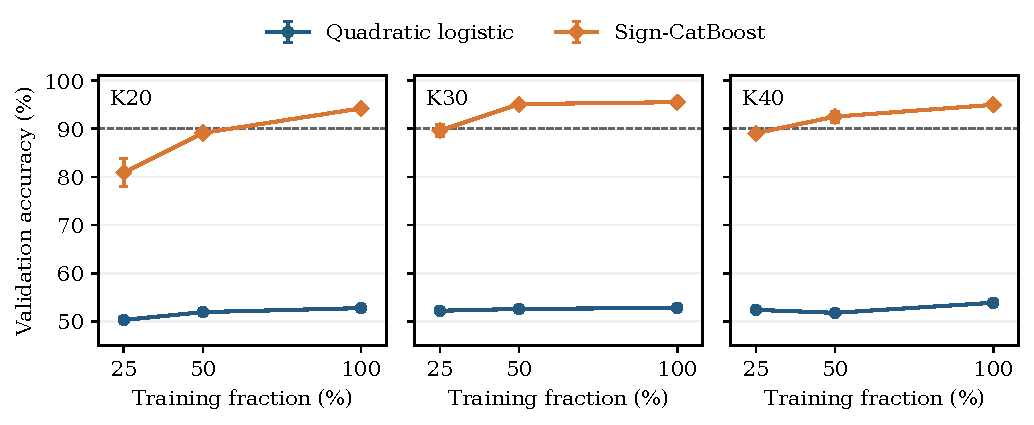
\includegraphics[width=\textwidth]{figures/learning_curves_3seed_layout.pdf}
\caption{Validation accuracy on matched nested training subsets. Both methods use the same rows at each fraction and the same fixed validation set. Full training sizes are 8,400, 14,000 and 22,400 for K20, K30 and K40. Points and error bars show mean and sample standard deviation over three model seeds on the same split. Quadratic logistic regression is deterministic. Lines guide the eye; the dashed line marks 90\%.}
\label{fig:scaling}
\end{figure*}

\section{Experimental Design}
\subsection{Partitions and evaluation roles}
We use the supplied labelled datasets and shared stratified 70/20/10 train/validation/local-test partitions, with split seed 67 (Table~\ref{tab:data}). The 70\% training partition is used for model fitting and CatBoost's internal cross-validation; the 20\% validation partition selects MLP width, LoRA rank and fixed refit epochs, and compares CatBoost with the selected MLP. These choices are locked before this local rerun's test evaluation. The selected configurations are refitted on the combined 90\% training and validation rows, with data-dependent preprocessing fitted only on those rows. The 10\% local test set was previously inspected during group development, so its scores should be interpreted as development evidence rather than a pristine independent estimate. Classification accuracy is the primary metric, and the original paper's 90\% target is a reference.


\begin{table}[t]
\centering
\caption{Shared labelled-data partitions. The adaptation task has 40 input dimensions. Each separate hidden set has 10,000 unlabelled examples.}
\begin{tabular}{lrrr}\toprule
Dataset & Train & Validation & Local test \\\midrule
K20 & 8,400 & 2,400 & 1,200 \\
K30 & 14,000 & 4,000 & 2,000 \\
K40 & 22,400 & 6,400 & 3,200 \\
K40-Adapt & 2,800 & 800 & 400 \\\bottomrule
\end{tabular}
\label{tab:data}
\end{table}

For the final comparison, all trainable models were refitted locally on the combined training and validation partitions using a macOS arm64 CPU. CatBoost, the MLP, the linear probe and LoRA use training seeds 42, 123 and 2026; numerical training uses one CPU thread. CatBoost's configuration was selected through fresh K20 training-only three-fold cross-validation and held fixed across datasets. Its outer-validation mean accuracy exceeded that of the selected MLP on all three main datasets. Validation selected MLP width 256 throughout; its fixed refit durations are 48, 49 and 18 epochs for K20, K30 and K40, respectively. LoRA ranks 1, 2, 4 and 8 use 22, 19, 14 and 13 epochs, respectively; the linear probe uses 33 epochs. Each duration is the median of that configuration's three locally selected validation epochs and is held constant across the three refits. Rank 1 was selected by the highest mean validation accuracy, with lower mean validation loss and then lower rank breaking ties. The MLP and adaptation models predict class 1 when the logit exceeds zero. Means and sample standard deviations describe training-seed variability on one fixed test split; majority classification, L-BFGS logistic regression and zero-shot inference are deterministic here. For the required hidden predictions, the selected CatBoost and rank-1 LoRA configurations are separately fitted on all labelled rows with seed 42; hidden labels are unavailable, so no hidden-set accuracy is claimed.

\subsection{Hypotheses and controlled comparisons}
\textbf{H1: Alternative learning methods can overcome the limitations of polynomial classifiers.} Kryptonite-3.0 reports that polynomial logistic regression fails to reach its 90\% accuracy target, even with high-degree feature expansion. We investigate whether this limitation extends to other learning approaches by comparing majority, linear and quadratic logistic baselines with sign-transformed CatBoost and MLPs trained from scratch. Sign-based CatBoost tests a binary feature representation combined with gradient-boosted trees.

\textbf{H2: The benefits of additional training data depend on the learning procedure.} Kryptonite-3.0 observes only marginal improvements when increasing the training data for quadratic logistic regression. To examine whether this finding generalizes, we compare its learning curve with that of sign-transformed CatBoost. Both methods are trained on identical nested subsets containing 25\%, 50\%, and 100\% of the available training data and evaluated on the same validation set, with hyperparameters fixed across training sizes. The subsets use seed 42. This comparison evaluates complete learning procedures, including model architecture and input representation.

\textbf{H3: LoRA can improve KryptoNet-40 adaptation beyond frozen-representation baselines.} Kryptonite-3.0 reports poor performance from zero-shot inference and frozen-feature probing, leaving adaptation of the pretrained hidden layers unexplored. We investigate whether updating these representations can improve downstream performance by comparing zero-shot KryptoNet-40, linear probing, and LoRA with ranks $(r\in\{1,2,4,8\})$ on Kryptonite-40-Adapt. Each trainable configuration is evaluated across three random seeds. LoRA adapts the hidden layers while retaining and training the pretrained output head, whereas the linear probe reinitializes its head and keeps the hidden layers frozen.





\begin{table*}[t]
\centering
\caption{Local-test accuracy (\%) after fitting each trainable method on 90\% of the labelled data. Entries are mean $\pm$ sample standard deviation across three seeds on one fixed split. Majority and L-BFGS logistic regression are deterministic, with identical repetitions.}
\begin{tabular}{lrrr}\toprule
Method & K20 & K30 & K40 \\\midrule
Majority & $50.42 \pm 0.00$ & $50.05 \pm 0.00$ & $50.19 \pm 0.00$ \\
Linear logistic & $49.58 \pm 0.00$ & $48.95 \pm 0.00$ & $48.84 \pm 0.00$ \\
Quadratic logistic & $53.92 \pm 0.00$ & $54.50 \pm 0.00$ & $53.41 \pm 0.00$ \\
Sign-CatBoost & $93.44 \pm 0.05$ & $96.28 \pm 0.25$ & $96.24 \pm 0.05$ \\
MLP (width 256) & $92.36 \pm 0.55$ & $93.95 \pm 0.23$ & $94.82 \pm 0.30$ \\
\bottomrule
\end{tabular}
\label{tab:main}
\end{table*}

\begin{figure*}[t]
\centering
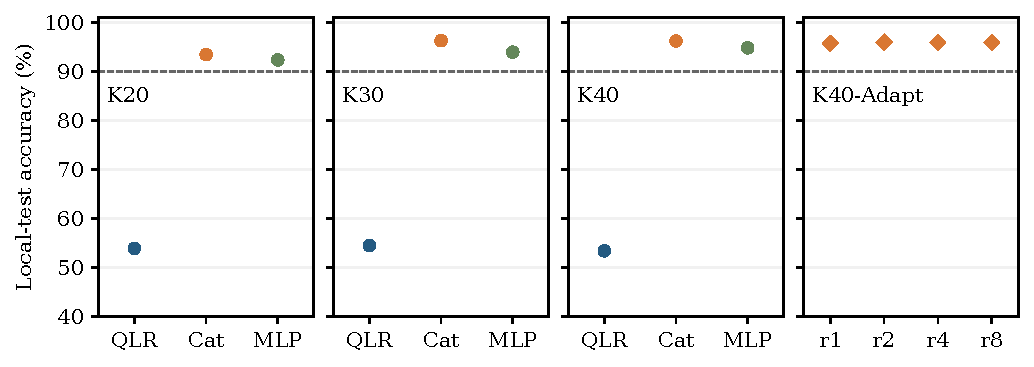
\includegraphics[width=\textwidth]{figures/test_3seed_layout.pdf}
\caption{Local-test accuracy after refitting on the combined training and validation partitions. Quadratic logistic regression, sign-CatBoost and the MLP are shown for K20, K30 and K40; the right panel shows LoRA ranks on K40-Adapt. Points and error bars show mean and sample standard deviation over three seeds on one split. The dashed line marks 90\%.}
\label{fig:refit}
\end{figure*}

\begin{table}[t]
\centering
\caption{K40-Adapt local-test accuracy on 400 examples, reported as mean $\pm$ sample standard deviation across three seeds. Trainable models use 3,600 training and validation rows. Zero-shot is deterministic; its repeated predictions are identical.}
\begin{tabular}{lrr}\toprule
Method & Trainable params & Accuracy (\%) \\\midrule
Zero-shot & 0 & $49.00 \pm 0.00$ \\
Linear probe & 513 & $48.33 \pm 0.52$ \\
LoRA $r=1$ & 4,137 & $95.75 \pm 0.25$ \\
LoRA $r=2$ & 7,761 & $96.00 \pm 0.25$ \\
LoRA $r=4$ & 15,009 & $95.92 \pm 0.14$ \\
LoRA $r=8$ & 29,505 & $95.92 \pm 0.14$ \\
\bottomrule
\end{tabular}
\label{tab:adapt}
\end{table}

\section{Experimental Results}
\subsection{Alternative classifiers exceed the polynomial controls}
Sign-CatBoost achieves mean local-test accuracies of 93.44\%, 96.28\% and 96.24\% on Kryptonite-20, -30 and -40, respectively (Table~\ref{tab:main}). Its class-1 F1 means are 93.37\%, 96.30\% and 96.24\%. Quadratic logistic regression obtains 53.92\%, 54.50\% and 53.41\% accuracy, while the selected width-256 MLP obtains 92.36\%, 93.95\% and 94.82\%. CatBoost was chosen for the three main datasets using validation means before this local-test rerun.

\subsection{Matched learning curves}
Figure~\ref{fig:scaling} compares identical nested training subsets. At 50\% of the original training partition, mean sign-CatBoost validation accuracy is 89.12\%, 95.12\% and 92.53\% for K20, K30 and K40. Increasing the subset from 25\% to 100\% improves sign-CatBoost by 13.32, 5.92 and 5.89 percentage points, versus 2.46, 0.60 and 1.47 points for quadratic logistic regression. The methods differ in both classifier and representation, so these curves compare complete learning procedures rather than isolating a single causal factor.

\subsection{LoRA permits adaptation with few trainable parameters}
On the 400-example K40-Adapt local test, zero-shot inference obtains 49.00\% and the refitted linear probe obtains 48.33\% mean accuracy. LoRA ranks 1, 2, 4 and 8 obtain 95.75\%, 96.00\%, 95.92\% and 95.92\%, respectively (Table~\ref{tab:adapt}). Rank 1 was selected by the fresh validation study, which recorded 96.33\% mean accuracy for that rank. It trains 4,137 parameters (0.51\% of KryptoNet-40) and uses 66.85\% of the counted full-fine-tuning matrix operations per training step. Rank 2 exceeds rank 1 by 0.25 percentage points on the 400-example local test, equivalent to one correct prediction; the validation-based choice remains rank 1. Figure~\ref{fig:refit} compares the locally refitted models across all four tasks.

\section{Discussion}
\subsection{Revisiting Kryptonite-3.0's inferences}
Sign-CatBoost and the MLP exceed 90\% mean local-test accuracy on all three main Kryptonite datasets. The matched curves show that additional data can help the tested CatBoost procedure more than quadratic logistic regression, and LoRA updates the pretrained hidden layers effectively on K40-Adapt. These observations contradict extending the mock paper's failures of selected procedures to every learning approach. Universal approximation is an existence statement; successful optimization and generalization with finite data require separate evidence.

The local test uses one fixed split and had been inspected during earlier group development. The new selection was validation-based, but that history limits claims of independent confirmation. Training-seed standard deviations do not quantify uncertainty across new data splits, and the hidden challenge labels remain unavailable.

\subsection{Further experiments}
Repeated outer splits would characterize performance across data partitions. Matched head-initialization, learning-rate and layer-placement experiments would further compare adaptation strategies.

\newpage
\subsection{Environmental impact}
The fresh experiments were run on a macOS arm64 CPU without a GPU; CatBoost and PyTorch training used one numerical thread. Run-level fitting times are recorded with the experiment outputs. The validation-selected rank-1 LoRA configuration trains 0.51\% of KryptoNet-40's parameters and uses 66.85\% of full fine-tuning's counted matrix operations per training step (Section~2.5). These operation counts do not directly measure energy use; no hardware power measurements were collected.

\begin{samepage}
\subsection{Conclusion}
The fresh local experiments show over 90\% mean local-test accuracy for sign-CatBoost and the MLP on K20, K30 and K40, model-dependent gains from additional training data, and effective low-rank adaptation of KryptoNet-40. Validation-selected rank-1 LoRA reaches 95.75\% mean local-test accuracy while training 0.51\% of its parameters. The hidden sets require separate evaluation.

\end{samepage}

\begin{thebibliography}{9}
\bibitem[Hu et al.(2022)]{hu2022}
Hu, E. J., Shen, Y., Wallis, P., Allen-Zhu, Z., Li, Y., Wang, S., Wang, L., \& Chen, W. (2022).
LoRA: Low-rank adaptation of large language models.
In \emph{International Conference on Learning Representations}.
\url{https://arxiv.org/abs/2106.09685}.

\bibitem[Kingma \& Ba(2015)]{kingma2015}
Kingma, D. P., \& Ba, J. (2015).
Adam: A method for stochastic optimization.
In \emph{International Conference on Learning Representations}.
\url{https://arxiv.org/abs/1412.6980}.

\newpage
\bibitem[Leshno et al.(1993)]{leshno1993}
Leshno, M., Lin, V. Y., Pinkus, A., \& Schocken, S. (1993).
Multilayer feedforward networks with a nonpolynomial activation function can approximate any function.
\emph{Neural Networks}, \emph{6}(6), 861--867.
\url{https://doi.org/10.1016/S0893-6080(05)80131-5}.

\bibitem[Needell et al.(2018)]{needell2018}
Needell, D., Saab, R., \& Woolf, T. (2018).
Simple classification using binary data.
\emph{Journal of Machine Learning Research}, \emph{19}(61), 1--30.
\url{https://jmlr.org/papers/v19/17-383.html}.

\bibitem[Prokhorenkova et al.(2018)]{prokhorenkova2018}
Prokhorenkova, L., Gusev, G., Vorobev, A., Dorogush, A. V., \& Gulin, A. (2018).
CatBoost: Unbiased boosting with categorical features.
In \emph{Advances in Neural Information Processing Systems} (Vol. 31).
\href{https://proceedings.neurips.cc/paper/2018/hash/14491b756b3a51daac41c24863285549-Abstract.html}{NeurIPS 2018 proceedings}.

\bibitem[Quinn \& Luther(2026)]{quinn2026}
Quinn, H., \& Luther, L. (2026).
\emph{Kryptonite-3.0: The final end to machine learning hype?}
Mathematics for Machine Learning coursework mock paper, Imperial College London.
\end{thebibliography}
\end{document}
